% Autor: Betti Oesterholz
% erstellt: 07.2010
% Dies ist der Handzettel zum fib-Projekt.
%
% Copyright (c) 2010 Betti Oesterholz
%
% Permission is granted to copy, distribute and/or modify this document
% under the terms of the GNU Free Documentation License, Version 1.2 or
% any later version published by the Free Software Foundation;
% with no Invariant Sections, no Front-Cover Texts, and no Back-Cover Texts.
%
% A copy of the license is included in the file ``fdl.tex'' .
%


\documentclass[10pt,a4paper]{article}
\pagestyle{empty} %keine Seitennummerierung
\usepackage{a4wide} % besser den Platz nutzen (kleinere R"ander)
\usepackage{ngerman} % Silbentrennung nach neuer Rechtschreibung
\usepackage[T1]{fontenc} % Type 1 Schriften
\usepackage{times} % Da die Standard-LaTeX-Schrift bei mir mit Acrobat nicht funkt.
\usepackage[ansinew]{inputenc} % Verwendung von Umlauten
%\usepackage{scrpage2} % Seitenformat
%\usepackage{titletoc}
%\usepackage{titlesec}
\usepackage{listings} % Programm-Listing
%\usepackage [usetoc]{titleref} 
\usepackage{graphicx} % Einbindung von Graphiken
\usepackage{url} % URLs durch \url{}
%\usepackage{bibgerm} % deutsche Bibliographie
%\usepackage{txfonts}%Paket fr das nat Symbol
\usepackage{multicol}
%\usepackage{makeidx}%for the index
%\usepackage{longtable}
%\usepackage{amsmath}%mathematikumgebung {equation*} usw.
\usepackage{picinpar}%Textumflossene Bilder

% Seitenstil festlegen
%\pagestyle{useheadings}%or: headings

% naehste vier Zeilen: Format des Inhaltsverzeichnisses
%\titlespacing{\section}{0pt}{5cm}{5cm}%spacing by sections {in front}{above}{below}
%\dottedcontents{section}[1.5em]{\addvspace{1.0em}}{1.3em}{0.7pc}
%\dottedcontents{subsection}[3.8em]{}{2.2em}{0.7pc}
%\dottedcontents{subsubsection}[7.0em]{}{3.1em}{0.7pc}

%\setcounter{secnumdepth}{4}%%nummerierung der Unterabschnitte bis Tiefe


%%%%%%%%%%%%%%%%%%%%%%%%%%%%%%%%%%%%%%%%%%%%%%%%%%%%%%%%%%%%%%%%%%%%%%%%%%%%%%%%%%%%%%%
% Definitionen fr das Verwenden von Listings

\newtheorem{Def}{Definition}

%%%%%%%%%%%%%%%%%%%%%%%%%%%%%%%%%%%%%%%%%%%%%%%%%%%%%%%%%%%%%%%%%%%%%%%%%%%%%%%%%%%%%%%
% Beginn des Dokuments
%\makeindex

\begin{document}

%\renewcommand{\sectionmark}[1]{\markboth{#1}{}}
%\pagenumbering {Roman}
%\automark{section}
%\pagestyle{scrheadings} % individ. Seitenlayout
%\setheadsepline{0.4pt}
%\ihead{} % Titelzeile innen
%\ohead{} % Titelzeile aussen
%\chead{\slshape \headmark}  % Titelzeile mitte
%\cfoot{\thepage} % Fusszeile mitte

% braucht man ein Inhaltsverzeichnis, so sind die naehsten drei Zeilen auszukommentieren
%\setcounter{tocdepth}{3}
%\tableofcontents
%\clearpage

% Vorschlag fr Titelzeile:
% Bei umfangreicheren Dokumenten
%\ihead{\slshape \headmark } % Darstellung von Sectionnummer und -name
%\ohead{}
%\chead{}


%\pagenumbering{arabic}

\ \vspace{-2.5cm}
\begin{center}
	\LARGE\bf Das Fib-Multimediasystem\\
\end{center}

\bigskip\noindent
Das Fib-Multimediasystem dient zum kodieren und speichern von Multimediadaten (z. B. Bildern oder Filme). Es zeichnet sich durch seine Universalit"at und Vielf"altigkeit aus.
\textbf{In diesem Sinne baut das Fib-Multimediasystem auf Vielfalt und nicht auf Spezialisierung auf.}

Dies bedingt auch eine hohe Komplexit"at, sowie viele Erweiterungs- und Verbesserungsm"oglichkeiten. Daher wird das Fib-System niemals wirklich fertig sein, sondern immer M"oglichkeiten f"ur weitere Verbesserungen bieten.


%\section{Komponenten}

Das Fib-System besteht aus mehreren Komponenten. Die wichtigsten werden im Nachfolgenden vorgestellt.

\section{Die Fib-Sprache}

\begin{window}[0,r,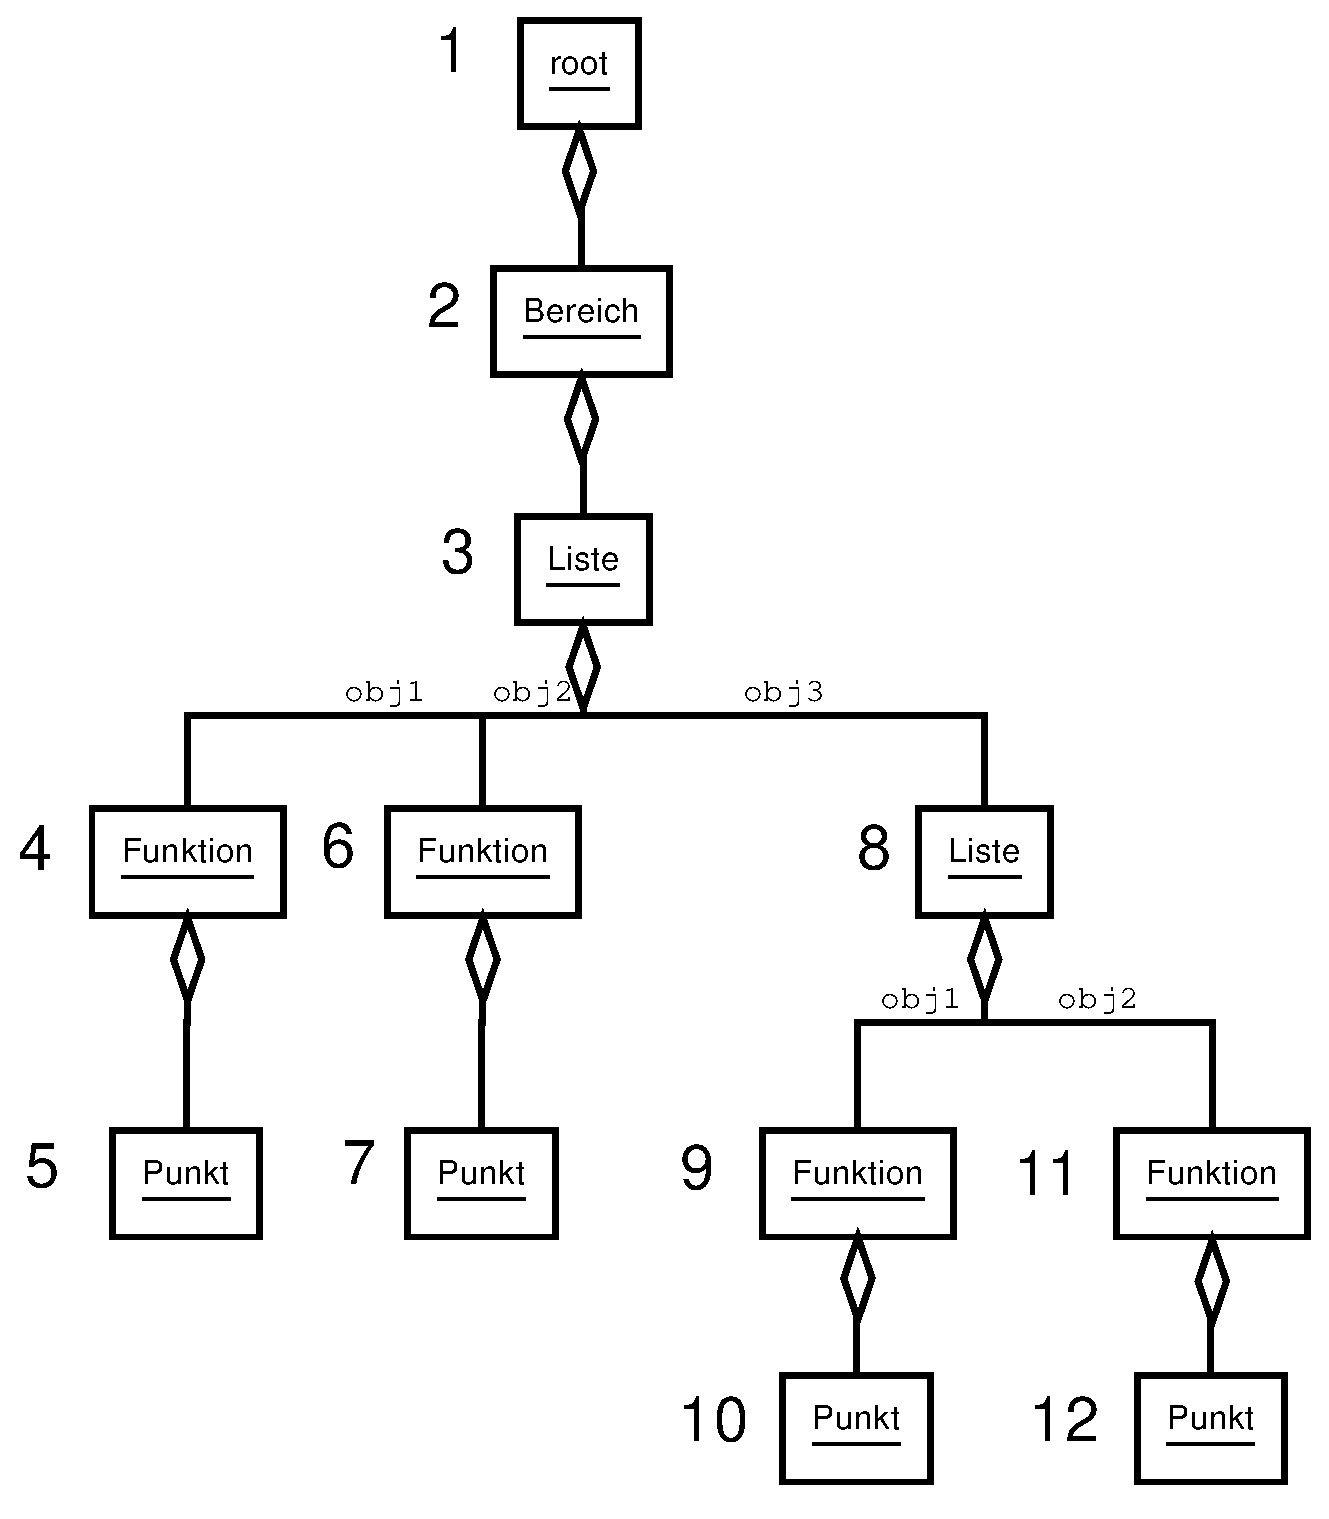
\includegraphics[scale=0.2]{./bilder/order_elements.eps},{}]
\noindent
Das Fib-Multimediaformat (die Fib-Sprache) dient zum Speichern von Multimediainformationen in strukturierter, funktionaler und hierarchischer Form. Die Struktur des Fib-Multi\-media\-for\-mats unterst"utzt die Objektsicht auf Dinge. Das Fib-Format ist sehr m"achtig, da Ausdr"ucke kombiniert und verschachtelt werden k"onnen (Baukastensystem).
\textbf{Mit Fib ist die Frage nicht mehr, ob Sie etwas machen k"onnen, sondern nur noch, wie Sie etwas machen k"onnen.}
Der Speicheraufwand eines Multimediobjekts in Fib ist viel mehr von dessen Komplexit"at abh"angig als von dessen Gr"o"se (im Sinne von Ausdehnung in den Dimensionen, also beispielsweise die Anzahl der Punkte bei Bildern), wie bei "ublichen Speicherformaten.

Die einzige Einschr"ankung bez"uglich der Multimediadaten, die im Fib-Format darstellbar sind, ist, dass sie als Eigenschaften von Punkten eines endlichen, euklidischen und diskreten (es gibt kleinste Einheiten) Raumes darstellbar sind. Daher k"onnen nicht nur Bilder und T"one mit Fib abgespeichert werden, sondern beispielsweise auch Ger"uche oder wie weich etwas ist.
\end{window}

Als Grundger"ust von Fib-Multimediadaten dient ein Baum. Die Bl"atter sind Endpunkte, die f"ur die Darstellung von bzw. Zuordnung zu Punkten oder Teilmultimediaobjekten dienen. In den "Asten und der Ausrichtung dieser werden Darstellungsparameter oder Eigenschaften der Bl"atter kodiert.
%Alt: In den "Asten und der Ausrichtung dieser, welche z. B. am weitesten links stehen, werden Darstellungsparameter oder Eigenschaften der Bl"atter kodiert, z. B. wie oft es dargestellt wird und mit welcher Farbe.


\section{Der genetische Algorithmus}

\begin{window}[0,l,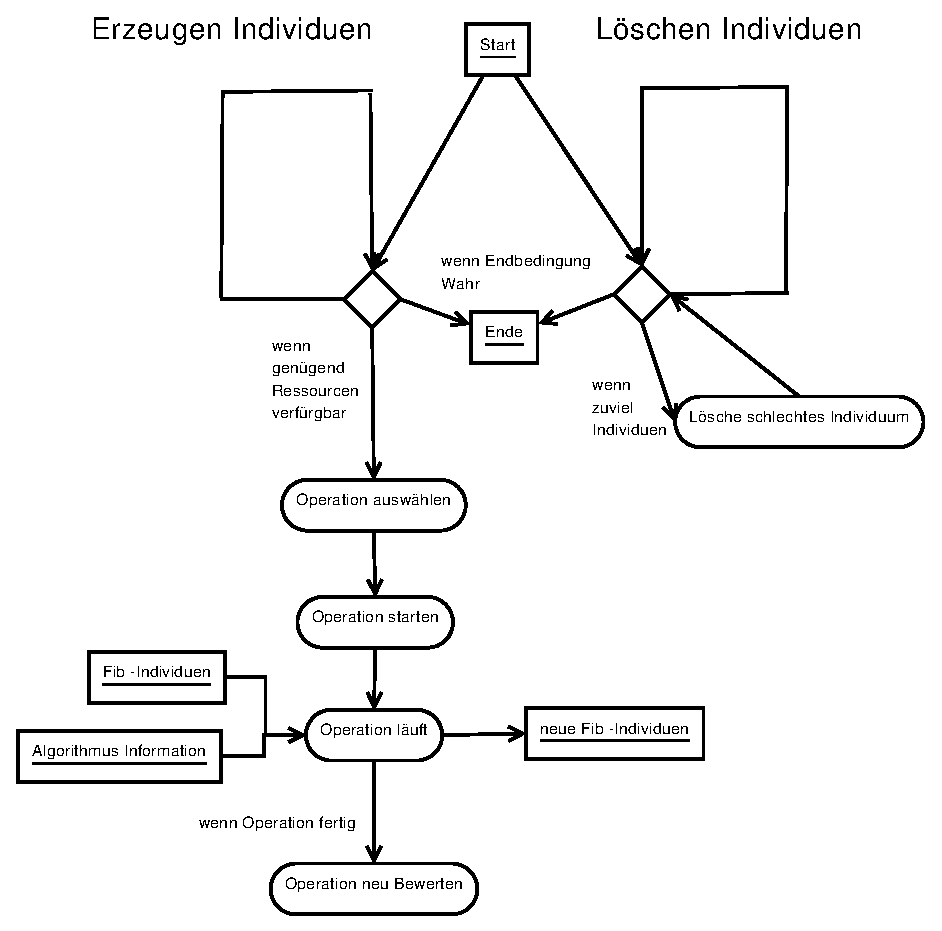
\includegraphics[scale=0.3]{./bilder/algorithmus.eps},{}]
\noindent
Die zweite wichtige Komponente des Fib-Systems ist der genetische Algorithmus zum Kodieren in und Komprimieren von Fib-Multi\-media\-objekten. Der gro"se Vorteil dessen ist, dass die Kodierung und Komprimierung nicht mehr an einem bestimmten Algorithmus gebunden ist, sondern dass die eigentlichen Kodierungs- und Komprimierungsalgorithmen im genetischen Algorithmus als Operatoren eingebunden werden, welche leicht hinzugef"ugt und ge"andert werden k"onnen. Dadurch ist es leicht, neue Kodierungs- und Komprimierungsideen einzubringen und eine Vielzahl von diesen auf ein Multimediaobjekt anzuwenden.

In diesem Sinne ist der genetische Algorithmus f"ur Fib ein transgenialer Algorithmus, der darauf angelegt ist, die Ideen von Menschen zur Kodierung von Multimediadaten aus deren K"opfe herauszuholen und in einem Topf zu transportieren bzw. zu sammeln. Damit sollen diese Ideen/Algorithmen mehr leisten k"onnen, als es einzelne k"onnten.
\end{window}
Der Algorithmus kann damit mehr Intelligenz in sich vereinen, als es ein Mensch (oder auch eine kleine Gruppe) hervorbringen kann.


\section{Konvertierungsprogramme}

Die Konvertierungsprogramme f"ur Fib dienen zur "Ubersetzung von anderen Multimediaformaten in das Fib-Multimediaformat und andersherum. Bei dieser "Ubersetzung sind auch einige Optimierungen der Zielmultimediadaten m"oglich.



\end{document}







